\documentclass[paper=a4wide, fontsize=10pt]{scrartcl}	 % A4 paper and 11pt font size
\usepackage[portuguese]{babel}
\usepackage{booktabs}
\usepackage{amssymb}
\usepackage[svgnames]{xcolor} % Using colors
\usepackage{background} % To include background images
\usepackage{amsmath}
\usepackage{fancyhdr} % Needed to define custom headers/footers
\usepackage[a4paper, left=20mm, right=20mm, top=20mm, bottom=2cm, footskip=1.2cm]{geometry}  % Changing size of document
%\usepackage[square, numbers, comma, sort&compress]{natbib} % Use the natbib reference package - read up on this to edit the reference style; if you want text (e.g. Smith et al., 2012) for the in-text references (instead of numbers), remove 'numbers'
\newcommand*\dif{\mathop{}\!\mathrm{d}}
\newcommand{\naturais}{\mathbb{N}}
\newcommand{\reais}{\mathbb{R}}
\newcommand{\Esp}[1]{\mathbb{E}[#1]}
\newcommand{\EspMonstro}[1]{\mathbb{E}\Bigg[#1\Bigg]}
\newcommand{\Vari}[1]{\mathbb{V}\text{ar}[#1]}
\newcommand{\VariMonstro}[1]{\mathbb{V}\text{ar}\Bigg[#1\Bigg]}
\newcommand{\Estim}[1]{\hat{#1}}
\newcommand{\Norm}[2]{\mathcal{N}(#1#2)}
\newcommand{\Vies}[1]{\mathbb{B}[#1]}
\newcommand{\Prob}[1]{\mathbb{P}(#1)}
\newcommand{\ProbMonstro}[1]{\mathbb{P}\Bigg(#1\Bigg)}
\newcommand{\Cova}[1]{\mathbb{C}\text{ov}[#1]}
\newcommand{\CovaMonstro}[1]{\mathbb{C}\text{ov}\Bigg[#1\Bigg]}
\usepackage[alf]{abntex2cite}  % Citações padrão ABNT
\usepackage{braket}
\usepackage{float}

%%%%%% Setting up the style

\setlength\parindent{0pt} % Gets rid of all indentation
\backgroundsetup{contents={
\includegraphics[width=\textwidth]{logo.jpg}},scale=0,placement=top,opacity=1,position={7.2cm,2cm}} %  OIST Logo
\pagestyle{fancy} % Enables the custom headers/footers

\lhead{} \rhead{} % Headers - all  empty

\definecolor{emerald}{RGB}{0,155,119}
\definecolor{RedHeat}{RGB}{152,0,46}
\definecolor{EgyptianBlue}{RGB}{2,45,180}


\title{\vspace{-1.8cm}  \color{emerald} Relatório de Pesquisa - EAE0324}
\subtitle{Análise da influência racial sobre o Salário: PNAD COVID % Title of the rotation project
\vspace{-1.0cm} }
\date{} % No date

\lfoot{\color{EgyptianBlue} Guilherme Dias Vianna}  % Write your name here
\rfoot{\color{RedHeat} IME-USP}


\renewcommand{\headrulewidth}{0.0pt} % No header rule
\renewcommand{\footrulewidth}{0.4pt} % Thin footer rule

%%%%%% Starting the document

\begin{document}

\maketitle % Print the title
\thispagestyle{fancy} % Enabling the custom headers/footers for the first page


% In the following lines, add the relevant information
\vspace{-1.5cm} \textbf{Nome:} Guilherme Dias Vianna

\textbf{NUSP:} 9301429

\textbf{Data de Entrega:} 27 de Novembro de 2023

\textbf{Professora:} Solange Ledi Gonçalves

\textbf{Unidade:} FEA - USP

\section{Introdução}

    O presente trabalho tem como objetivo avaliar o efeitos da raça no salário dos brasileiros em um modelo no mesmo espírito de Mincer em \cite{doi:10.1086/258055}. É feita uma análise da influência da raça (e do gênero) sobre a remuneração, controlando por várias covariáveis já apontadas como significativas na literatura. Posteriormente é feito um teste de diagnóstico mais próprio da Estatística do que da Econometria para verificarmos se as hipóteses de modelo linear clássico são válidas.


\section{Motivação/Revisão da Literatura}
    \subsection{Diferenças no salário entre raças e gênero}
    A literatura especializada (tanto nacional quanto internacional) em economia do trabalho tem vários estudos de caso investigando tais relações entre raça/gênero e seus efeitos sobre a remuneração de pessoas comparáveis, citamos por exemplo \cite{Salardi2012WageDA}, \cite{madalozzo_2010}  e a meta-análise de \cite{https://doi.org/10.1111/j.0950-0804.2005.00256.x}

\section{Metodologia}
    \subsection{Escolha do Modelo}
    Nosso modelo populacional consistirá de uma relação log-lin da forma:
    \begin{equation}
        \log(\mathbf{y}) = \boldsymbol{\beta} \mathbf{X}+\mathbf{u}
    \end{equation}

    Aqui, \(\mathbf{y}\) é nossa variável-resposta, \(\boldsymbol{\beta}\) nosso vetor de parâmetros, \(\mathbf{X}\) nossa matriz de observações amostrais e por fim \(\mathbf{u}\) é nosso vetor de erros aleatórios, que está sujeito as hipóteses do \textbf{modelo linear clássico}:

    \begin{equation}\label{MLC}
        \mathbf{u} \sim \boldsymbol{\mathcal{N}}(\mathbf{0},\boldsymbol{\Sigma})
    \end{equation}

    \begin{equation}\label{COV}
        \Cova{\mathbf{X}_i,\mathbf{u}} = 0
    \end{equation}

    Com \(\boldsymbol{\Sigma}\) uma matriz de variância-covariância desconhecida.
    
    \subsection{Escolha de variáveis de controle}

    Escolhemos o seguinte subconjunto de dados da PNAD Covid para compôr \(\mathbf{X}\):

    \begin{table}[ht]
\centering
\begin{tabular}{@{}lll@{}}
\toprule
Variável     & Descrição                          & Tipo e valores assumidos \\ \midrule
Educação         & Nível de educação                  & Categórica (0 = sem ensino superior, 1 c.c)         \\
Região         & Subregião da família                  & Categórica (0 = Nordeste, 1 = Sudeste)          \\
Situação         & Distinção entre o domicílio urbano e rural                  & Categórica (0 = Rural, 1 = Urbano)               \\
Raça         & Cor da pele                  & Categórica ( 0 = não-branca, 1 = branca)           \\
Condição         & Condição entendida na estrutura do domicílio                  & Categórica (1 = Responsável pelo domicílio, 0 c.c) \\
Idade         & Idade do entrevistado                  & Contínua (\(\in (0,130)\))      \\
logsal         & logaritmo em base 10 do salário                  & Contínua \((\in(0,+\infty))\)            \\
 \bottomrule
\end{tabular}
\caption{Descrição das variáveis explicativas}
\label{tab:minha_tabela}
\end{table}

Como investigação preliminar, podemos ver como essas variáveis estão correlacionadas:

\begin{figure}[H]
\centering
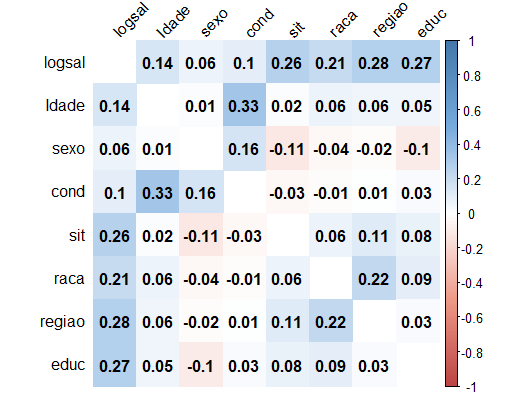
\includegraphics[width=0.5\linewidth]{MatrizCorrelação.png}
\caption{Matriz de correlação entre as variáveis de interesse.}
\end{figure}

\section{Resultados e Teste de Robustez}

    \subsection{Resultados}

    Nossa regressão gera as seguintes estimativas para cada uma das variáveis (e \(\kappa\) para o intercepto):
    \begin{table}[H]
        
% Table created by stargazer v.5.2.3 by Marek Hlavac, Social Policy Institute. E-mail: marek.hlavac at gmail.com
% Date and time: sáb, nov 25, 2023 - 22:59:30
\begin{table}[!htbp] \centering 
  \caption{} 
  \label{} 
  \begin{tabular}{@{\extracolsep{5pt}}lcccc} 
  \\[-1.8ex]\hline 
  \hline \\[-1.8ex] 
   & Coeficiente & Erro Padrão & p-valor & \(t\) \\ 
  \hline \\[-1.8ex] 
   Região & 0.142$^{***}$ & (0.002) & \(\otimes\) & 59.322 \\ 
   Raça& 0.097$^{***}$ & (0.002) & \(\otimes\) & 39.577 \\ 
   Condição & 0.042$^{***}$ & (0.002) & \(\otimes\) & 17.109 \\ 
   Situação & 0.210$^{***}$ & (0.003) & \(\otimes\) & 71.134 \\ 
   Educação & 0.449$^{***}$ & (0.005) & \(\otimes\) & 87.219 \\ 
   Idade & 0.002$^{***}$ & (0.0001) & \(\otimes\) & 24.186 \\ 
   Sexo & 0.082$^{***}$ & (0.002) & \(\otimes\) & 34.254 \\ 
   \(\kappa\) & 2.671$^{***}$ & (0.005) & \(\otimes\) & 554.150 \\ 
  \hline \\[-1.8ex] 
  Número de Observações & \multicolumn{4}{c}{78,851} \\ 
  R$^{2}$ & \multicolumn{4}{c}{0.241} \\ 
  Estatística F & \multicolumn{4}{c}{3570.356$^{***}$} \\ 
  \hline 
  \hline \\[-1.8ex] 
  \end{tabular} 
\end{table}



    \end{table}
    \textbf{Legenda:} O símbolo \(\otimes\) daqui pra frente é utilizado para sinalizar que a estatística calculada é menor que \(10^{-12}\)\\

Veja que, dada a hipótese (\ref{MLC}), todos as nossas estimativas são estatisticamente significativas a 1\% (com certeza o número alto de observações contribui para isso). O sinal dos regressores também mostra um gap salarial (\textit{ceteris paribus}) entre brancos e não brancos (em linha com a literatura).
Também é visto um prêmio salarial no ensino superior, também observado na literatura de forma bem recorrente. Raciocínios idênticos seguem para as variáveis de Região e Situação, também corroborando outros efeitos já documentados.
Nosso modelo tem um R\(^2\) de 0.241, ou seja este modelo reproduz 24\% da variabilidade dos nossos dados.
\newpage



    \subsection{Análise de Subgrupos}

    Separando nossa base por gênero temos para observações de homens:
    
    \begin{table}[H]
        
% Table created by stargazer v.5.2.3 by Marek Hlavac, Social Policy Institute. E-mail: marek.hlavac at gmail.com
% Date and time: sáb, nov 25, 2023 - 22:59:30
\begin{table}[!htbp] \centering 
  \caption{} 
  \label{} 
  \begin{tabular}{@{\extracolsep{5pt}}lcccc} 
  \\[-1.8ex]\hline 
  \hline \\[-1.8ex] 
   & Coeficiente & Erro Padrão & p-valor & \(t\) \\ 
  \hline \\[-1.8ex] 
   Região & 0.158$^{***}$ & (0.003) & \(\otimes\) & 51.460 \\ 
   Raça & 0.090$^{***}$ & (0.003) & \(\otimes\) & 28.367 \\ 
   Condição & 0.077$^{***}$ & (0.003) & \(\otimes\) & 24.155 \\ 
   Situação & 0.220$^{***}$ & (0.004) & \(\otimes\) & 62.011 \\ 
   Educação & 0.510$^{***}$ & (0.008) & \(\otimes\) & 63.021 \\ 
   Idade & 0.002$^{***}$ & (0.0001) & \(\otimes\) & 18.522 \\ 
   \(\kappa_h\) & 2.671$^{***}$ & (0.006) & \(\otimes\) & 554.150 \\ 
  \hline \\[-1.8ex] 
  Número de Observações & \multicolumn{4}{c}{46,008} \\ 
  R$^{2}$ & \multicolumn{4}{c}{0.266} \\ 
  Estatística F & \multicolumn{4}{c}{2777.565$^{***}$} \\ 
  \hline 
  \hline \\[-1.8ex] 
  \end{tabular} 
\end{table}


    \end{table}

    E para mulheres:
    
    \begin{table}[H]
        
% Table created by stargazer v.5.2.3 by Marek Hlavac, Social Policy Institute. E-mail: marek.hlavac at gmail.com
% Date and time: sáb, nov 25, 2023 - 22:59:31
\begin{table}[!htbp] \centering 
  \caption{} 
  \label{} 
  \begin{tabular}{@{\extracolsep{5pt}}lcccc} 
  \\[-1.8ex]\hline 
  \hline \\[-1.8ex] 
   & Coeficiente & Erro Padrão & p-valor & \(t\) \\ 
  \hline \\[-1.8ex] 
   Região & 0.116$^{***}$ & (0.004) & \(\otimes\) & 30.819 \\ 
   Raça & 0.103$^{***}$ & (0.004) & \(\otimes\) & 27.045 \\ 
   Condição & -0.007$^{*}$ & (0.004) & 0.074 & -1.787 \\ 
   Situação & 0.196$^{***}$ & (0.005) & \(\otimes\) & 37.480 \\ 
   Educação & 0.408$^{***}$ & (0.007) & \(\otimes\) & 60.862 \\ 
   Idade & 0.002$^{***}$ & (0.0002) & \(\otimes\) & 13.922 \\ 
   \(\kappa_m\) & 2.724$^{***}$ & (0.005) & \(\otimes\) & 351.977 \\ 
  \hline \\[-1.8ex] 
  Número de Observações & \multicolumn{4}{c}{32,843} \\ 
  R$^{2}$ & \multicolumn{4}{c}{0.211} \\ 
  Estatística F & \multicolumn{4}{c}{1466.090$^{***}$} \\ 
  \hline 
  \hline \\[-1.8ex] 
  \end{tabular} 
\end{table}

    \end{table}

    Veja que, embora ambas as tabelas mostrem efeitos similares em termos de significância e sinal para a variável Raça, a variável Condição no caso feminino é menos estatisticamente significante e apresenta uma diminuição da remuneração.
    
    \subsection{Envelope Simulado}
    Por mais que nossos resultados até agora tenham sido estatisticamente significativos, uma boa parte disso se apoia somente em (\ref{MLC}), faremos um envelope simulado (nos baseando em \cite{f9cc0d93-2781-3c61-a795-5084da4ba2e1} e \cite{Atkinson}, com uma implementação de \cite{Everitt}) para verificar se nosso modelo e hipótese de normalidade são adequados.

    O procedimento segue em linhas gerais como:
    \begin{enumerate}
    \item Gerar \( n \) observações \( \mathcal{N}(0, 1) \)
    \item Rodar regressões como nosso modelo com cada uma dessas observações
    \item Obter resíduos padronizados \(t_i\) (studentizados) para cada uma das regressões.
    \item Repetir os passos (1)-(3) \( m \) vezes, gerando os resíduos \( t_{ij}^* \), para \( i = 1, \ldots, n \) e \( j = 1, \ldots, m \).
    \item Ordenar cada grupo de \( n \) resíduos para obter \( t_{(1)j}^* \leq \ldots \leq t_{(n)j}^* \).
    \item Obter os limites \( t_{(i)l}^* = \min\{t_{(i)1}^*, \ldots, t_{(i)m}^*\} \) e \( t_{(i)s}^* = \max\{t_{(i)1}^*, \ldots, t_{(i)m}^*\} \) e a mediana \( t_{(i)M}^* = \text{mediana}\{t_{(i)1}^*, \ldots, t_{(i)m}^*\} \). 
    \item Juntar \( (t_{(1)l}^*, \ldots, t_{(n)l}^*), (t_{(1)M}^*, \ldots, t_{(n)M}^*), (t_{(1)s}^*, \ldots, t_{(n)s}^*) \) formando, respectivamente, o limite inferior, a mediana e o limite superior do envelope.

    Se os resíduos observados caírem fora do envelope, isso sugere que o modelo pode estar mal especificado, indicando possíveis violações das hipóteses (como homoscedasticidade, não-normalidade). Isso sugere que devemos ser muito mais céticos com nossas conclusões anteriores

\end{enumerate}

Vejamos que, para \(n\) sendo nosso número de observações original e \(m=50\), temos a seguinte distribuição de resíduos e o envelope com 95\% de confiança.

\begin{figure}[H]
\centering
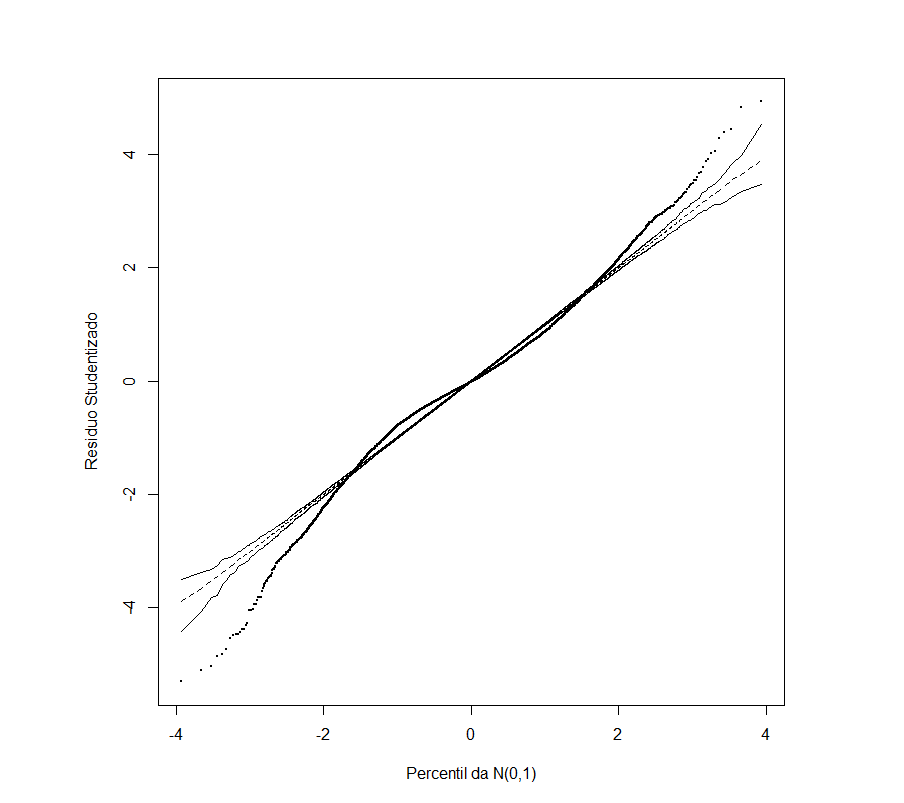
\includegraphics[width=0.8\linewidth]{Rplot01.png}
\caption{Resultados do envelope simulado.}
\end{figure}

Veja que, infelizmente nosso modelo parece estar mal especificado, com uma distribuição de resíduos bem pouco dentro do envelope esperado.

Seria interessante observamos outras famílias possíveis para modelar \(\mathbf{u}\) e assim recalcularmos a significância estatística das estimativas, para termos uma noção mais acurada do efeito que está sendo observado.
\section{Conclusão}

Encerramos então com o diagnóstico de que, embora nosso modelo reproduza resultados apoiados pela literatura com uma alta significância, provavelmente persistem problemas de especificação no modelo que precisarão ser analisados com mais calma e que deixam as conclusões anteriores bem menos certeiras. São necessárias então novas análises com modelos mais robustos e outras hipóteses sobre os erros para que obtenhamos estimativas e p-valores robustos, caso os mesmos sobrevivam à novas rodadas de testes como os feitos aqui.

\bibliography{Bibliografia}



\end{document}
